
\exercise{Model Learning}
The new and improved Spinbot 2000 is a multi-purpose robot platform.
It is made of a kinematic chain consisting of a linear axis $q_{1}$, a rotational axis $q_{2}$ and another linear axis $q_{3}$, as shown in the figure below.
These three joints are actuated with forces and torques of $u_{1}$, $u_{2}$, and $u_{3}$.
Different end effectors, including a gripper or a table tennis racket, can be mounted on the end of the robot, indicated by the letter $E$.
Thanks to Spinbot's patented SuperLight technology, the robot's mass is distributed according to one point mass of $m_{1}$ at the second joint and another point mass of $m_{2}$ at the end of the robot $E$.

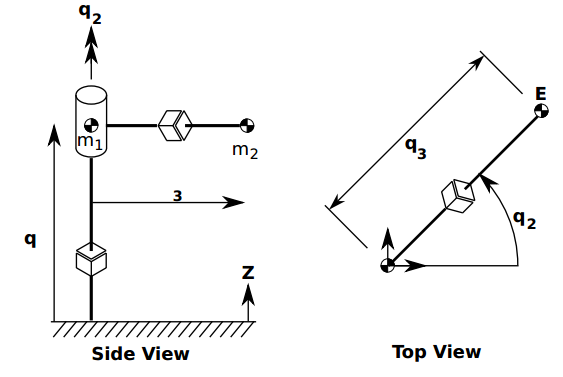
\includegraphics[width=0.5\textwidth]{img/spinbot.png}

The inverse dynamics model of the Spinbot is given as
\begin{align*}
u_{1} &= (m_{1}+m_{2})(\ddot{q}_{1}+g),\\
u_{2} &= m_{2}(2\dot{q}_{3}\dot{q}_{2}q_{3}+q_{3}^{2}\ddot{q}_{2}),\\
u_{3} &= m_{2}(\ddot{q}_{3}-q_{3}\dot{q}_{2}^{2}).
\end{align*}
We now collected 100 samples from the robot while using a PD controller with gravity compensation at a rate of 500Hz.
The collected data (see \texttt{spinbotdata.txt}) is organized as follows\\
\begin{tabular}{| l || c | c | c | l  }
  \hline
   & $t_1$ & $t_2$ & $t_3$ & \ldots\\
  \hline
  \hline
  $q_{1}[m]$ &  &  &  & \\
  \hline
  $q_{2}[rad]$ &  &  &  & \\
  \hline
  $q_{3}[m]$ &  &  &  & \\
  \hline
  \ldots &  &  &  &  \\
  \hline
  $\ddot{q}_{3}[m/s^{2}]$ &  &  &  & \\
  \hline
  $u_{1}[N]$ &  &  &  & \\
  \hline
  $u_{2}[Nm]$ &  &  &  & \\
  \hline
  $u_{3}[N]$ &  &  &  & \\
  \hline
\end{tabular}

Given this data, you want to learn the inverse dynamics of the robot to use a model-based controller.
The inverse dynamics of the system will be modeled as $\vec{u}=\vec{\phi}(\vec{q},\dot{\vec{q}},\ddot{\vec{q}})^{\T}\vec{\theta}$, where $\vec{\phi}(\vec{q},\dot{\vec{q}},\ddot{\vec{q}})$ are features and $\vec{\theta}$ are the parameters.

\begin{questions}

%----------------------------------------------

\begin{question}{Problem Statement}{2}
What kind of machine learning problem is learning an inverse dynamics model? What kind of information do you need to solve such a problem?

\begin{answer}
	Theory:\\
	Learning Inverse Dynamics is quite interesting, as rigid body("Starrk\"orper") dynamics are lacking of good friction models and are therefore incomplete. Moreover dynamic parameters are difficult to estimate. The task of an inverse model is to predict the action needed to reach a desired state. This means a Inverse Matrix can be learned directly.
	
	Inverse Dynamics: $u=f(q,\dot{q},\ddot{q}_{ref}), \quad \dddot{q}_t^{des}=K_P(q_t^{des}-q_t)+K_D(\dot{q}_t^{des}-\dot{q}_t)$ (PD-Controller)
	
	Task:\\
	Kind of machine learning problem:\\
	Learning an inverse dynamics model is a kind of supervised learning (in model learning) which can be solved by linear regression. It should be noted that only if the system is an invertible function an inverse dynamics model can be learned.

	
	Kind of information:\\
	To learn an inverse dynamics model you need many measurements of the output values and input values. For the inverse model above the output values are: ($u_i$) and the input values are: ($q_i, \dot{q}_i,...$).


	\end{answer}

\end{question}

%----------------------------------------------


\begin{question}{Assumptions}{5}
Which standard assumption has been violated by taking the data from trajectories?

\begin{answer}
	The data of the trajectories should be Independent and identically distributed(IID). 

	A collection of random variables is IID if each random variable has the same probability distribution as the others and all are mutually independent.

	\end{answer}

\end{question}

%----------------------------------------------


\begin{question}{Features and Parameters}{4}
Assuming that the gravity $g$ is unknown, what are the feature matrix $\vec{\phi}$ and the corresponding parameter vector $\vec{\theta}$ for $\vec{u}=[u_{1},u_{2},u_{3}]^{\T}$?
(Hint: you do not need to use the data at this point)

\begin{answer}
	
	What are the parameters?
		
		\begin{align*}
		u_{1} &= (m_{1}+m_{2})(\ddot{q}_{1}+g),\\
		u_{2} &= m_{2}(2\dot{q}_{3}\dot{q}_{2}q_{3}+q_{3}^{2}\ddot{q}_{2}),\\
		u_{3} &= m_{2}(\ddot{q}_{3}-q_{3}\dot{q}_{2}^{2}).
		\end{align*}
		
	$\underset{3\times 1}{y_1}= \phi^T \theta=  \underset{3\times 3} {\begin{bmatrix}
	\ddot{q_1}&0&1\\0&2\dot{q_3}\dot{q_2}q_3+q_3^2\ddot{q_2}&0\\0&\ddot{q_3}-q_3 \dot{q_2}^2&0
	\end{bmatrix}}
	\underset{3\times 1}{\begin{bmatrix}
	m_1+m_2\\m_2\\ m_2g+m_1g
	\end{bmatrix}}$
	
	For n measurements: \\
	$\underset{3n \times 1}Y=\begin{bmatrix}
	y_1\\...\\y_n
	\end{bmatrix}$
	
	$\underset{3n \times 3}\Phi=\begin{bmatrix}
	\phi_1^T\\...\\ \phi_n^T
	\end{bmatrix}$
	
	Linear Regression:\\
	$\underset{3 \times 1}\theta = ( \underset{3\times 3n}{\Phi^T} \; \underset{3n \times 3}{ \Phi})^{-1} \underset{3 \times 3n}\Phi^T \underset{3n \times 1}{Y}$

	\end{answer}

\end{question}

%----------------------------------------------


\begin{question}{Learning the Parameters}{2}
You want to compute the parameters $\vec{\theta}$ minimizing the squared error between the estimated forces/torques and the actual forces/torques.
Write down the matrix equation that you would use to compute the parameters. For each matrix in the equation, write down its size.\\
Then, compute the least-squares estimate of the parameters $\vec{\theta}$ from the data and report the learned values.

\begin{answer}
	
	Task:\\
	$min_{\theta} \sum_{i=1}^n (u_{meas,i}-u_{pred,i})^2 =min_{\theta} \sum_{i=1}^n (u_{meas,i}-\phi^T_i \theta)^2 $
	
		$\underset{3 \times 1}\theta = ( \underset{3\times 3n}{\Phi^T} \; \underset{3n \times 3}{ \Phi})^{-1} \underset{3 \times 3n}\Phi^T \underset{3n \times 1}{Y}$
		
theta: [  1.57600862   1.65617664  15.09760938]

g: 9.57964898326

m1: -0.0801680184959

m2: 1.65617663934
	
	
	\end{answer}

\end{question}

%----------------------------------------------


\begin{question}{Recovering Model Information}{4}
	Can you recover the mass properties $m_{1}$ and $m_{2}$ from your learned parameters? Has the robot learned a plausible inverse dynamics model? Explain your answers.
	
\begin{answer}
	Yes the masses and the g could be derived see d). No the robot has apparently not learned a plausible inverse dynamics model, cause all masses should be at least higher than zero and g should be around 9.81 . 
	\end{answer}
\end{question}

%----------------------------------------------


\begin{question}{Model Evaluation}{7}
Plot the forces and torques predicted by your model over time, as well as those recorded in the data and comment the results. Is the model accuracy acceptable? If not, how would improve your model? Use one figure per joint.

\begin{answer}


\begin{minipage}{1\textwidth}
	\begin{center}
		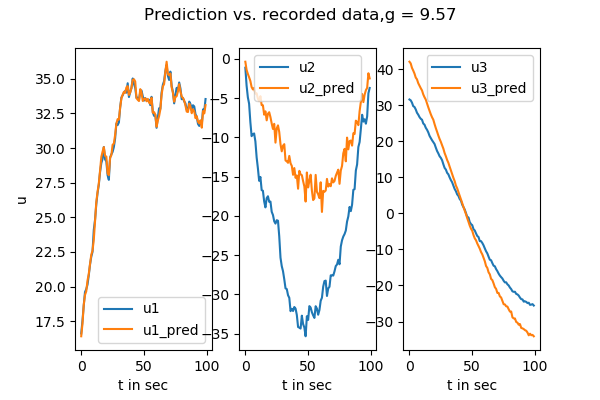
\includegraphics[width=1\textwidth]{img/1f-g_wrong.png} 
		\captionof{figure}{Predicted values for u}
	\end{center}
\end{minipage} \hfill

	The Model accuracy is especially for the torque $u_2$ not acceptable (see middle figure above). The reason therefore is that the mass $m_1$ is obviously wrong. That is why the trajectory of the torque $u_2$ is overestimated. 
	
	Model Improvement:
	The model could be improved, by assuming g to be 9.81. Next the masses can be predicted again using: 
	
		$\underset{3\times 1}{y_1}= \phi^T \theta=  \underset{3\times 2} {\begin{bmatrix}
			\ddot{q_1}+g&0\\0&2\dot{q_3}\dot{q_2}q_3+q_3^2\ddot{q_2}\\0&\ddot{q_3}-q_3 \dot{q_2}^2
			\end{bmatrix}}
	\underset{2\times 1}{\begin{bmatrix}
			m_1 +m_2\\m_2
		\end{bmatrix}}$
	
	Another method may be to use many different trajectories and use them all to predict the parameters. Than you have better distributed data and less over-fitting.
	
\end{answer}

\end{question}

%----------------------------------------------


\begin{question}[bonus]{Models for Control}{4}
Name and describe three different learned models types and their possible applications.
\end{question}
\begin{answer}

\begin{tabular}{|p{4cm}|p{7cm}|p{5cm}|}
		\hline
		Model Type&Description  &Possible Application \\
		\hline
				Forward Model &Predict the future state: $s_{k+1}=f_D(s_k,u_k)+\epsilon$s:state, u:action Can be used for direct action geneartion.  &Usefull for long-term predictions. Can be used as Simulator.
			\\	\hline
			Inverse Model &Predict the action needed to reach a desired state or other outcome. $u=\pi(s_t)=f(s_t,s_{t+1}^{des})$. An Inverse can be learned directly (e.g. inverse dynamics control). Only if system is an invertable function, inverse model learning is useful.&In inverse dynamics control: The action u to reach a desired state with $q_t^{des}, \dot{q_t^{des}},\ddot{q_t^{des}}$ should be predicted. Applications are Model Based Control and Fast Forward control. 	 \\	 \hline 

		Mixed Model&Predict required task elements with a forward model and use an inverse model for control.&Systems with Hysteresis, Inverse Kinematics. \\  \hline
		
		Multi-Step Prediction Model&Predict a task variable long term (far in the future). Especially useful for system's which have a lot of latency in the control loop.                                      &Throw a ball into a cup at a given position (like the example in the lab). Or Systems with a lot latency like the Mars Rover when controlling it from earth.  \\ \hline
\end{tabular}
	
	\end{answer}



%----------------------------------------------

\end{questions}
